\documentclass[a4paper,11pt]{article}
\usepackage{graphicx}
\usepackage{float}
\usepackage{subfig}
\usepackage{geometry}
\usepackage{amsmath,amssymb}
\usepackage{amsthm}
\usepackage{bbold}
\usepackage{mathtools}
\usepackage{braket}
\usepackage{booktabs}
\usepackage[table,xcdraw]{xcolor}
\usepackage[utf8]{inputenc}
\usepackage{cite}
\usepackage[english]{babel}
\usepackage{lipsum}
\usepackage{setspace}
\usepackage{minted}
\usepackage{xcolor}
\newcommand{\R}{\mathbb{R}}
\usepackage{hyperref}
\hypersetup{colorlinks=true,linkcolor=blue}
\geometry{a4paper, top=2.5cm, bottom=2.5cm, left=3cm, right=2.5cm}

\begin{document}
	\author{Catalano Giuseppe, Cerrato Nunzia}
	\title{Numerical Linear Algebra Homework Project 4:\\Unconstrained Optimization}
	\date{}
	\maketitle
	
	\noindent In this project we want to perform unconstrained optimization using the Newton method both in its standard form and by considering its variants which make use of the backtracking and the trust region approach. We will apply these methods to four test functions and we will compare these approaches to see how convergence changes.
	
\section{Algorithms}
\begin{minted}[mathescape, linenos, breaklines]{python}
def Newton(func, grad, hess, tol, maxit, x_0, sol_x, sol_f, alpha=1, sigma=0.0001, rho=0.5, backtracking=False):
    r''' This function implements the standard Newton method for unconstrained optimization.

     Parameters
     ----------
     func : function
         Function to be minimized. It must be :math:`f : \mathbb{R}^{n} \rightarrow \mathbb{R}`
     grad : function
         Gradient of the function. It returns a 1d-array (vector)
     hess : function
         Hessian of the function. It returns a 2d-array (matrix)
     tol : float
         Tolerance parameter for the stopping criterion
     maxit : int
         Maximum number of iterations
     x_0 : ndarray
         Starting point
     sol_x : ndarray
         Exact solution (x) to the minimization problem
     sol_f : float
         Exact minimum value of the function
     alpha : float
         Step lenght. Default value alpha=1
     sigma : float
         Constant parameter in :math:`(0,1)`. Used if backtracking = True. Default value sigma=0.0001
     rho : float
         Reduction parameter in :math:`(0,1)`. Used if backtracking = True. Default value rho=0.5

     Results
     -------
     results : dict
         Dictonary of the results given by the function. It contains the following items:
           - 'convergence' : (bool) True if the algorithm converges, False if it doesn't converge
           - 'k' : (int) final iteration at which convergence is reached
           - 'min_point' : (ndarray) computed point at which the minimum of the function is reached
           - 'min_value' : (float) computed minimum value of the function
           - 'interm_point' : (list) list of the intermediate points
           - 'error_x' : (list) list that contains the 2-norm of the difference between each intermediate point and the exact solution (min_point). 
           - 'error_f' : (list) list that contains the difference between the function evaluated at each intermediate point and its value in the exact minimum point
           - 'scalar_product' : (list) list that contains the scalar product between the descent direction and the gradient

     '''
old_point = x_0
alpha_0 = alpha

# Create a list to save intermediate points
interm_points = [old_point]
# Create a list to save the scalar product between the gradient and the descent direction
scalar_prod = []

new_point = x_0
# Cycle on the number of iterations
for k in range(maxit):
gradient = grad(old_point)
hessian = hess(old_point)

# Compute norms for the stopping criterion
norm_grad = np_lin.norm(gradient)
norm_diff_x = np_lin.norm(new_point - old_point)

# Check if the stopping criterion is satisfied
if norm_grad <= tol and norm_diff_x <= tol*(1 + np_lin.norm(old_point)):            
min_value = func(new_point)
conv = True
print(k)
break

# Compute the descent direction by solving a linear system
p = np_lin.solve(hessian, -gradient)
scalar_prod.append(gradient@p)

# Implement backtracking if backtracking == True
if backtracking == True:
alpha = alpha_0
iteraz_backtracking = 0 
while func(old_point + alpha*p) > func(old_point) + (sigma*alpha)*(p @ gradient) \
and iteraz_backtracking < 100:
alpha = rho*alpha
iteraz_backtracking += 1         

# Compute the new point and add it to the list of intermediate points
new_point = old_point + alpha*p
interm_points.append(new_point)

old_point = new_point

if k == maxit-1:
min_value = func(new_point)
conv = False

gradient = grad(new_point)
hessian = hess(new_point)
p = np_lin.solve(hessian, -gradient)
scalar_prod.append(gradient@p)

# Compute the 2norm of the difference between each intermediate point and the exact solution
error_x = [np_lin.norm(interm_x - sol_x) for interm_x in interm_points]

# Compute the difference between the function evaluated in each intermediate point and 
# its value in the exact minimum point
error_f = [func(interm_x) - sol_f for interm_x in interm_points]

results = {'convergence': conv, 'k' : k, 'min_point' : new_point, 'min_value' : min_value ,
	'interm_point' : interm_points, 'error_x' : error_x, 'error_f' : error_f,
	'scalar_product' : scalar_prod}

return results

\end{minted}


	\section{Test Functions}
	dfbfd
	\subsection*{(a)}
	The first function that we want to consider is the following:
	\begin{equation}
		f(x_{1},x_{2}) = (x_{1}-2)^{4} + (x_{1}-2)^{2}x_{2}^{2} + (x_{2}+1)^{2}.
	\end{equation}
	This function assumes a minimum value, equal to $0$, in the point $(x_{1}^*,x_{2}^*)=(2,-1)$. We would like to obtain this minimum value by using the standard Newton algorithm implemented by the function ****Newton**** in the library ***Project\_4.py ****. We report below the gradient and the Hessian of $f$, which must be passed to the function ****Newton****.
	\begin{equation}
		\nabla f(x_{1},x_{2}) = \begin{bmatrix}
			4(x_{1}-2)^{3} + 2x_{2}^{2}(x_{1}-2)\\
			2x_{2}(x_{1}-2)^{2} + 2x_{2}(x_{2}-2)
		\end{bmatrix},
	\end{equation}

		\begin{equation}
		\nabla^{2} f(x_{1},x_{2}) = \begin{bmatrix}
			12(x_{1}-2)^{2} + 2x_{2}^{2} & 4x_{2}(x_{1}-2)\\
			4x_{2}(x_{1}-2) & 2(x_{1}-2)^{2} + 2
		\end{bmatrix}.
	\end{equation}
	
	\begin{table}
	\centering	
	\begin{tabular}{|c|c|c|c|}
		\hline
		k & $\| \textbf{x}_{k} - \textbf{x}^*\|_{2} $ & $f_{1}(\textbf{x}_{k}) - f_{1}(\textbf{x}^{*}) $ & $-\nabla f_{1}(\textbf{x}_{k})^{T} [\nabla^{2}f_{1}(\textbf{x}_{k})]^{-1} \nabla f_{1}(\textbf{x}_{k})$ \\
		\hline
		0 & $2.236$ & $6.000$ & $-9.000$ \\
		1 & $1.118$ & $1.500$ & $-1.761$ \\
		2 & $6.805\times10^{-1}$ & $4.092\times10^{-1}$ & $ -5.552\times10^{-1} $\\
		3 & $2.592\times10^{-1}$ & $6.489\times10^{-2} $ & $ -1.237\times10^{-1}$ \\
		4 & $5.012\times10^{-2}$ & $2.531\times10^{-3} $ & $ -5.026\times10^{-3}$ \\
		5 & $1.277\times10^{-3}$ & $1.632\times10^{-6}$ & $-3.262\times10^{-6}$ \\
		6 & $1.659\times10^{-6}$ & $2.754\times10^{-12}$ & $-5.508\times10^{-12}$\\
		7 & $1.404\times10^{-12}$ & $1.971\times10^{-24}$ & $-3.943\times10^{-24}$ \\
		\hline
	\end{tabular}
	\caption{$x_{0}=(1,1)^{T}$, Backtracking = False}
	\label{tab:table_a}
	\end{table}
	
	
	\begin{figure}[H]
		\centering
		\subfloat[][]{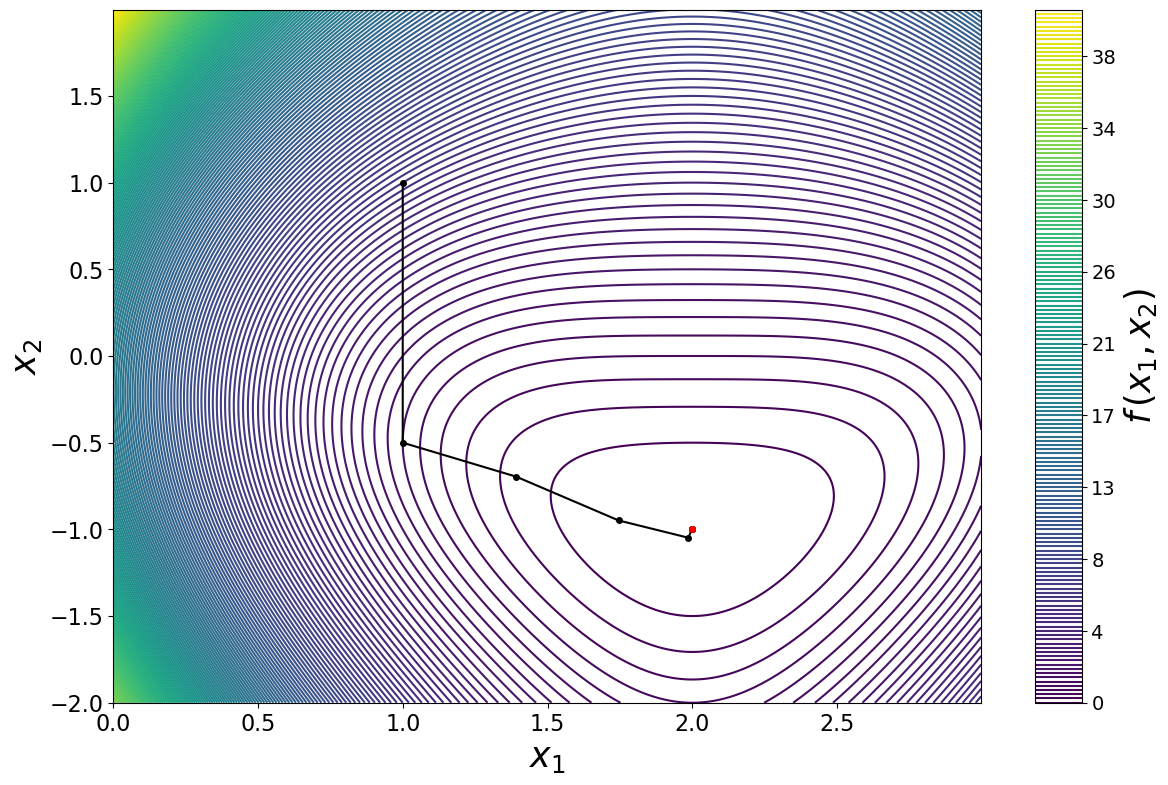
\includegraphics[scale=0.26]{Plot/func_a_standard_newton_contour.png}} \quad
		\subfloat[][]{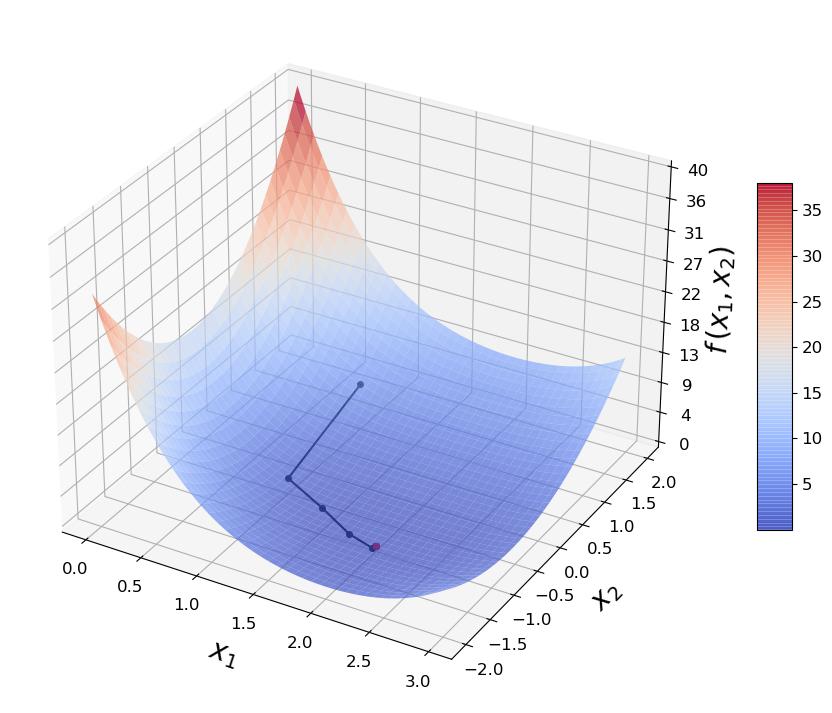
\includegraphics[scale=0.35]{Plot/func_a_standard_newton_3d.png}}
		\caption{Contour plot for the function $f^{(a)}(x_{1},x_{2})$ where the intermediate points are obtained by using the standard Newton method.}
		\label{Fig:func_a}
	\end{figure}

	\subsection{(b)}
	$f:\mathbb{R}^{4} \rightarrow  \mathbb{R}$, $f(\textbf{x}) = \textbf{b}^{T} + \frac{1}{2}\textbf{x}^{T}H\textbf{x}$
	\begin{equation}
		\textbf{b} = (5.04, -59.4, 146.4, -96.6)^{T}
	\end{equation}

	\begin{equation}
		H = \begin{bmatrix}
		0.16 & -1.2 & 2.4 & -1.4 \\
		-1.2 & 12.0 & -27.0 & 16.8 \\
		2.4 & -27.0 & 64.8 & -42.0 \\
		-1.4 & 16.8 & -42.0 & 28.0
		\end{bmatrix}
	\end{equation}

	\begin{table}[H]
		\centering
		\begin{tabular}{|c|c|c|c|}
			\hline
			k & $\| \textbf{x}_{k} - \textbf{x}^*\|_{2} $ & $f_{1}(\textbf{x}_{k}) - f_{1}(\textbf{x}^{*}) $ & $-\nabla f_{1}(\textbf{x}_{k})^{T} [\nabla^{2}f_{1}(\textbf{x}_{k})]^{-1} \nabla f_{1}(\textbf{x}_{k})$ \\
			\hline
			$0$ & $5.745$ & $5.223\times10^{2}$ & $-1.045\times10^{3}$ \\
			$1$ & $9.769\times10^{-13}$ & $2.842\times10^{-14}$ & $-9.948\times10^{-27}$ \\
			$2$ & $1.688\times10^{-13}$ & $0.000$ & $-2.005\times10^{-26}$ \\
			\hline
		\end{tabular}
	\end{table}

	\subsection{(c)}
	$f:\mathbb{R}^{2} \rightarrow  \mathbb{R}$, $f(x_{1},x_{2}) = (1.5 - x_{1}(1-x_{2}))^2 + (2.25 - x_{1}(1-x_{2}^{2}))^2 + (2.625 - x_{1}(1-x_{2}^{3}))^2 $
	
\begin{table}
	\centering
	\begin{tabular}{|c|c|c|c|}
		\hline
		k & $\| \textbf{x}_{k} - \textbf{x}^*\|_{2} $ & $f_{1}(\textbf{x}_{k}) - f_{1}(\textbf{x}^{*}) $ & $-\nabla f_{1}(\textbf{x}_{k})^{T}[\nabla^{2}f_{1}(\textbf{x}_{k})]^{-1} \nabla f_{1}(\textbf{x}_{k})$ \\
		\hline
		$0$ & $5.009$ & $8.17\times10^{1}$ & $-1.455\times10^{2}$ \\
		$1$ & $8.66\times10^{-1}$ & $2.423$ & $-4.527$ \\
		$2$ & $6.494\times10^{-2}$ & $2.407\times10^{-2}$ & $-4.643\times10^{-2}$ \\
		$3$ & $1.393\times10^{-1}$ & $3.45\times10^{-3}$ & $-6.32\times10^{-3}$ \\
		$4$ & $2.103\times10^{-2}$ & $1.383\times10^{-4}$ & $-2.704\times10^{-4}$ \\
		$5$ & $1.377\times10^{-3}$ & $2.863\times10^{-7}$ & $-5.717\times10^{-7}$ \\
		$6$ & $3.033\times10^{-6}$ & $2.186\times10^{-12}$ & $-4.372\times10^{-12}$ \\
		$7$ & $2.836\times10^{-11}$ & $1.233\times10^{-22}$ & $-2.466\times10^{-22}$ \\
		$8$ & $4.441\times10^{-16}$ & $4.437\times10^{-31}$ & $-8.79\times10^{-31}$ \\
		\hline
	\end{tabular}
	\caption{$x_{0}=(8,0.2)^{T}$, backtracking = False}
\end{table}

	\begin{figure}[h!]
		\centering
		\subfloat[][]{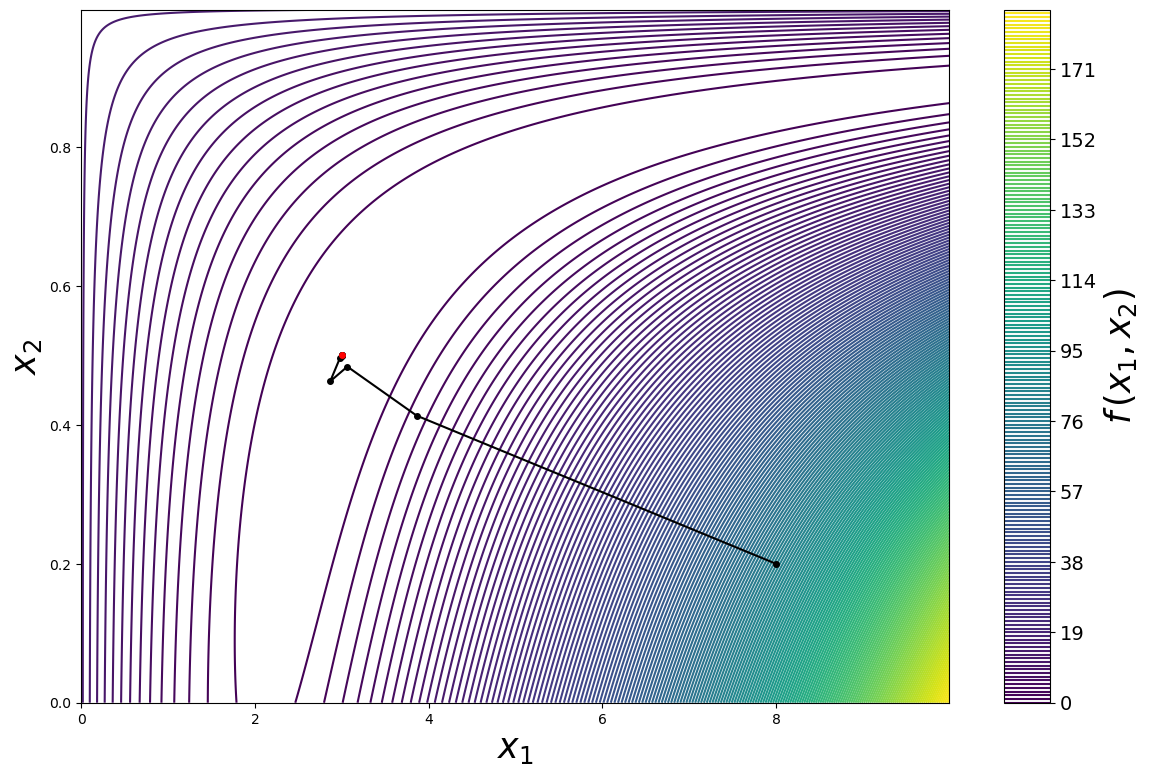
\includegraphics[scale=0.24]{Plot/func_c_standard_newton_x0_1_contour.png}} \quad
		\subfloat[][]{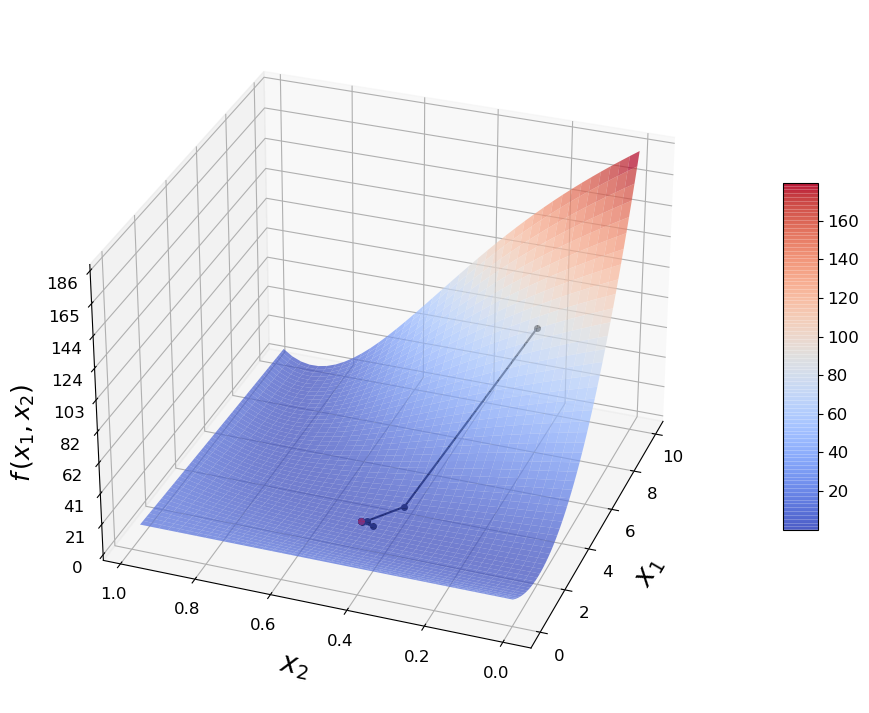
\includegraphics[scale=0.34]{Plot/func_c_standard_newton_x0_1_3d.png}}
		\caption{Contour plot and 3D plot for the function $f^{(c)}(x_{1},x_{2})$ where the intermediate points are obtained by using the standard Newton method $x_{0}=(0.75,-1.25)^{T}$.}
		\label{Fig:func_c}
	\end{figure}

	\begin{table}[H]
		\centering
		\begin{tabular}{|c|c|c|c|}
			\hline
			k & $\| \textbf{x}_{k} - \textbf{x}^*\|_{2} $ & $f_{1}(\textbf{x}_{k}) - f_{1}(\textbf{x}^{*}) $ & $-\nabla f_{1}(\textbf{x}_{k})^{T}[\nabla^{2}f_{1}(\textbf{x}_{k})]^{-1} \nabla f_{1}(\textbf{x}_{k})$ \\
			\hline
			$0$ & $5.009$ & $2.043$ & $-3.291$ \\
			$1$ & $3.963$ & $2.553\times10^{-1}$ & $-5.885\times10^{-2}$ \\
			$2$ & $4.218$ & $2.328\times10^{-1}$ & $-6.421\times10^{-1}$ \\
			$3$ & $1.661\times10^{1}$ & $5.743\times10^{2}$ & $-9.291\times10^{2}$ \\
			$4$ & $6.137$ & $5.226\times10^{1}$ & $-6.327\times10^{1}$ \\
			$5$ & $3.426$ & $1.596\times10^{1}$ & $-3.709$ \\
			$6$ & $2.974$ & $1.421\times10^{1}$ & $-8.445\times10^{-3}$ \\
			$7$ & $3.041$ & $1.42\times10^{1}$ & $-5.688\times10^{-8}$ \\
			$8$ & $3.041$ & $1.42\times10^{1}$ & $-1.083\times10^{-18}$ \\
			$9$ & $3.041$ & $1.42\times10^{1}$ & $0.000$ \\
			\hline
		\end{tabular}
		\caption{$x_{0}=(8,0.8)^{T}$, backtracking = False *** PROBLEMA? ***}
	\end{table}
	
	
	\begin{table}[H]
		\centering
		\begin{tabular}{|c|c|c|c|}
			\hline
			k & $\| \textbf{x}_{k} - \textbf{x}^*\|_{2} $ & $f_{1}(\textbf{x}_{k}) - f_{1}(\textbf{x}^{*}) $ & $-\nabla f_{1}(\textbf{x}_{k})^{T}[\nabla^{2}f_{1}(\textbf{x}_{k})]^{-1} \nabla f_{1}(\textbf{x}_{k})$ \\
			\hline
			$0$ & $5.009$ & $2.043$ & $-3.291$ \\
			$1$ & $3.963$ & $2.553\times10^{-1}$ & $-5.885\times10^{-2}$ \\
			$2$ & $4.218$ & $2.328\times10^{-1}$ & $-6.421\times10^{-1}$ \\
			$3$ & $2.920$ & $2.131\times10^{-1}$ & $-7.337\times10^{-2}$ \\
			$4$ & $2.471$ & $1.649\times10^{-1}$ & $-1.224\times10^{-1}$ \\
			$5$ & $1.340$ & $1.502\times10^{-1}$ & $-1.22\times10^{-1}$ \\
			$6$ & $1.192$ & $7.989\times10^{-2}$ & $-1.697\times10^{-1}$ \\
			$7$ & $6.453\times10^{-1}$ & $5.012\times10^{-2}$ & $-5.027\times10^{-2}$ \\
			$8$ & $3.335\times10^{-1}$ & $1.73\times10^{-2}$ & $-2.418\times10^{-2}$ \\
			$9$ & $8.357\times10^{-2}$ & $3.009\times10^{-3}$ & $-5.269\times10^{-3}$ \\
			$10$ & $2.128\times10^{-2}$ & $1.004\times10^{-4}$ & $-1.967\times10^{-4}$ \\
			$11$ & $2.767\times10^{-4}$ & $1.503\times10^{-7}$ & $-3.005\times10^{-7}$ \\
			$12$ & $1.103\times10^{-6}$ & $2.293\times10^{-13}$ & $-4.585\times10^{-13}$ \\
			$13$ & $2.404\times10^{-13}$ & $8.166\times10^{-25}$ & $-1.633\times10^{-24}$ \\
			$14$ & $0.000$ & $0.000$ & $0.000$ \\
			\hline
		\end{tabular}
	\caption{$x_{0}=(8,0.8)^{T}$, backtracking = True}
	\end{table}
	
	\subsection{(d)}
	$f:\mathbb{R}^{2} \rightarrow  \mathbb{R}$, $f(x_{1},x_{2}) = x_{1}^{4} + x_{1}x_{2} + (1+x_{2})^{2}$
	
	\begin{table}[H]
		\centering
		\begin{tabular}{|c|c|c|c|}
			\hline
			k & $\| \textbf{x}_{k} - \textbf{x}^*\|_{2} $ & $f_{1}(\textbf{x}_{k}) - f_{1}(\textbf{x}^{*}) $ & $-\nabla f_{1}(\textbf{x}_{k})^{T}[\nabla^{2}f_{1}(\textbf{x}_{k})]^{-1} \nabla f_{1}(\textbf{x}_{k})$ \\
			\hline
			$0$ & $1.119\times10^{-1}$ & $2.385\times10^{-2}$ & $-4.688\times10^{-2}$ \\
			$1$ & $4.601\times10^{-3}$ & $4.517\times10^{-5}$ & $-8.996\times10^{-5}$ \\
			$2$ & $2.951\times10^{-5}$ & $1.406\times10^{-9}$ & $-3.7\times10^{-9}$ \\
			$3$ & $3.805\times10^{-9}$ & $-4.436\times10^{-10}$ & $-6.372\times10^{-18}$ \\
			\hline
		\end{tabular}
	\caption{$x_{0}=(0.75,-1.25)^{T}$, $\alpha=1$, backtracking=False}
	\end{table}

	\begin{figure}[H]
		\centering
		\subfloat[][]{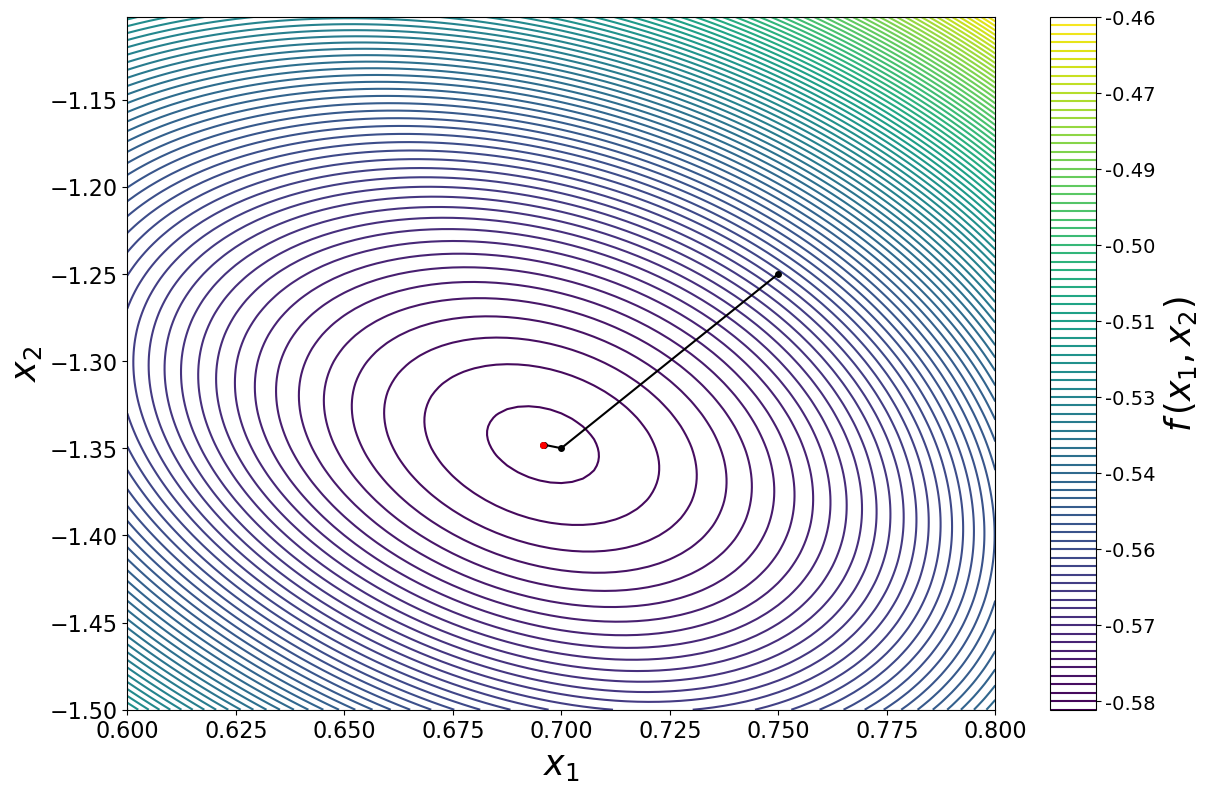
\includegraphics[scale=0.24]{Plot/func_d_standard_newton_x0_1_contour.png}} \quad
		\subfloat[][]{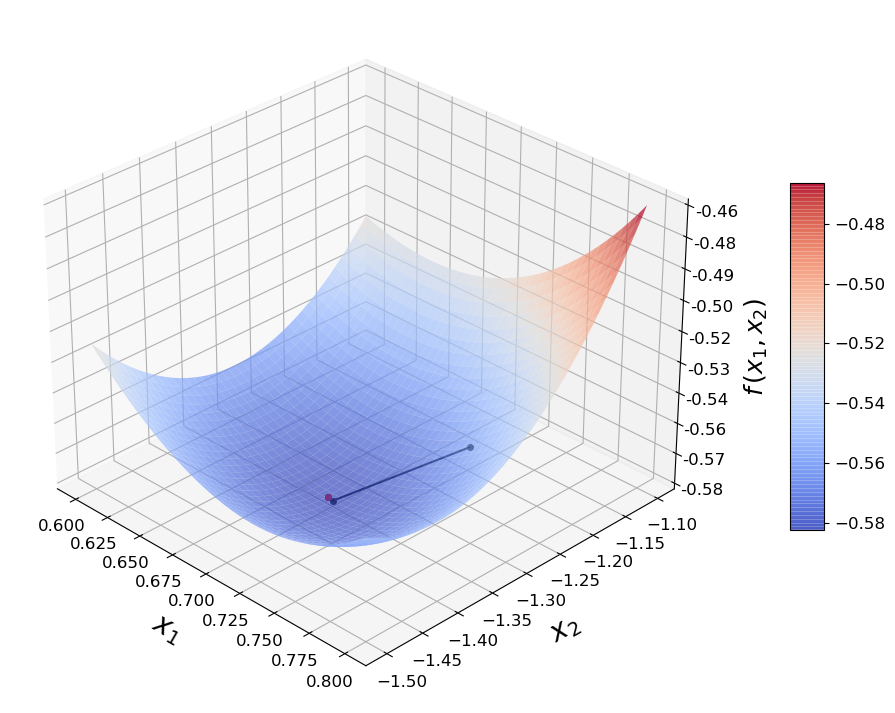
\includegraphics[scale=0.34]{Plot/func_d_standard_newton_x0_1_3d.png}}
		\caption{Contour plot and 3D plot for the function $f^{(d)}(x_{1},x_{2})$ where the intermediate points and the minimum point are obtained by using the standard Newton method with $alpha=1$. The starting point considered in this case is $x_{0}=(0.75,-1.25)^{T}$.}
		\label{Fig:func_d}
	\end{figure}

	\begin{table}[H] 
		\centering 
		\begin{tabular}{|c|c|c|c|} 
			\hline 
			k & $\| \textbf{x}_{k} - \textbf{x}^*\|_{2} $ & $f_{1}(\textbf{x}_{k}) - f_{1}(\textbf{x}^{*}) $ & $-\nabla f_{1}(\textbf{x}_{k})^{T}[\nabla^{2}f_{1}(\textbf{x}_{k})]^{-1} \nabla f_{1}(\textbf{x}_{k})$ \\
			\hline
			$0$ & $1.517$ & $1.582$ & $0.000$ \\
			$1$ & $2.837$ & $1.208\times10^{1}$ & $-1.432\times10^{1}$ \\
			$2$ & $2.181$ & $3.888$ & $-3.680$ \\
			$3$ & $1.725$ & $1.764$ & $-1.114$ \\
			$4$ & $1.352$ & $1.099$ & $-6.198\times10^{-1}$ \\
			$5$ & $8.656\times10^{-1}$ & $6.593\times10^{-1}$ & $2.174$ \\
			$6$ & $3.138$ & $2.143\times10^{1}$ & $-2.663\times10^{1}$ \\
			$7$ & $2.424$ & $6.213$ & $-6.657$ \\
			$8$ & $1.910$ & $2.391$ & $-1.830$ \\
			$9$ & $1.514$ & $1.320$ & $-6.987\times10^{-1}$ \\
			$10$ & $1.126$ & $8.791\times10^{-1}$ & $-1.402$ \\
			$11$ & $3.352\times10^{-1}$ & $3.219\times10^{-1}$ & $-5.271\times10^{-1}$ \\
			$12$ & $1.188\times10^{-1}$ & $3.348\times10^{-2}$ & $-6.1\times10^{-2}$ \\
			$13$ & $2.637\times10^{-2}$ & $1.514\times10^{-3}$ & $-2.957\times10^{-3}$ \\
			$14$ & $3.474\times10^{-3}$ & $2.572\times10^{-5}$ & $-5.128\times10^{-5}$ \\
			$15$ & $3.626\times10^{-4}$ & $2.789\times10^{-7}$ & $-5.586\times10^{-7}$ \\
			$16$ & $3.643\times10^{-5}$ & $2.375\times10^{-9}$ & $-5.637\times10^{-9}$ \\
			$17$ & $3.646\times10^{-6}$ & $-4.154\times10^{-10}$ & $-5.642\times10^{-11}$ \\
			$18$ & $3.659\times10^{-7}$ & $-4.434\times10^{-10}$ & $-5.643\times10^{-13}$ \\
			\hline
		\end{tabular}
		\caption{Table of data obtained using the standard Newton algorithm to minimize the function $f^{(d)}(x_{1},x_{2})$ by using $\alpha=0.9$ and by considering as starting point $x_{0}=(0,0)^{T}$.}
	\end{table}

	
	\begin{figure}[H]
		\centering
		\subfloat[][]{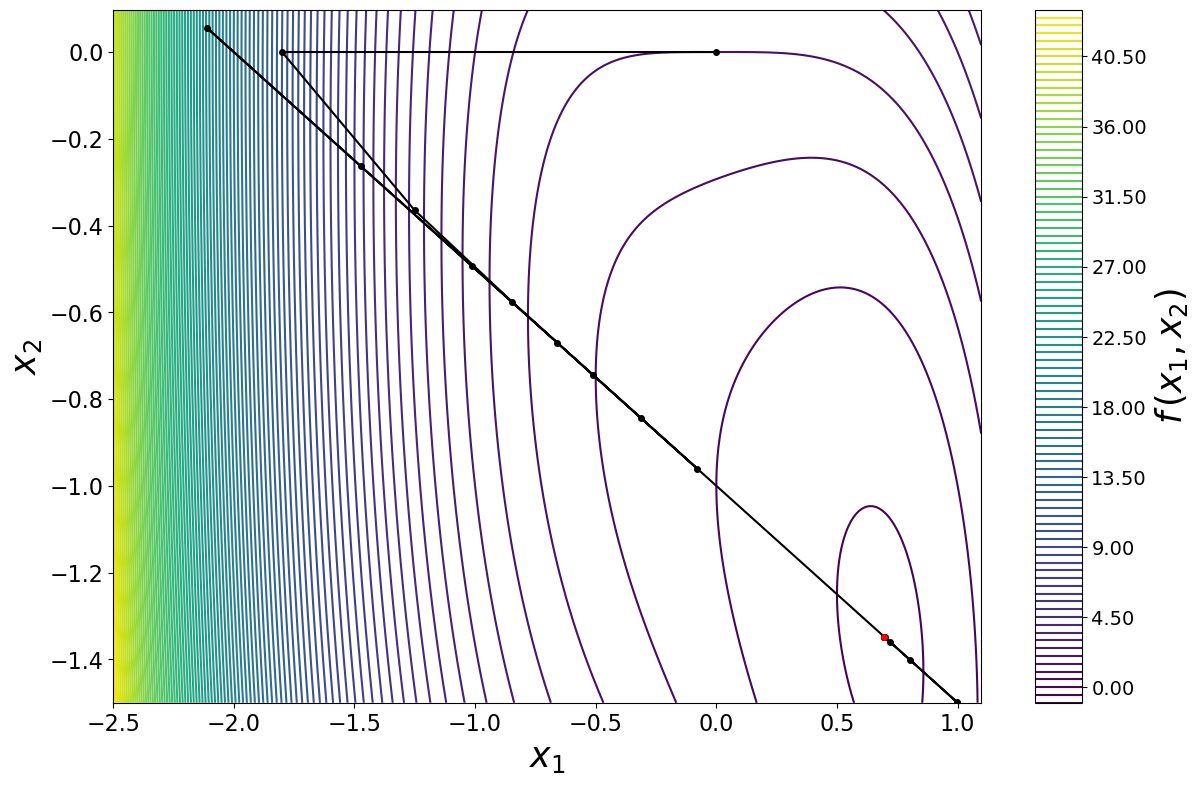
\includegraphics[scale=0.24]{Plot/func_d_standard_newton_x0_2_alpha=0.9_contour.png}} \quad
		\subfloat[][]{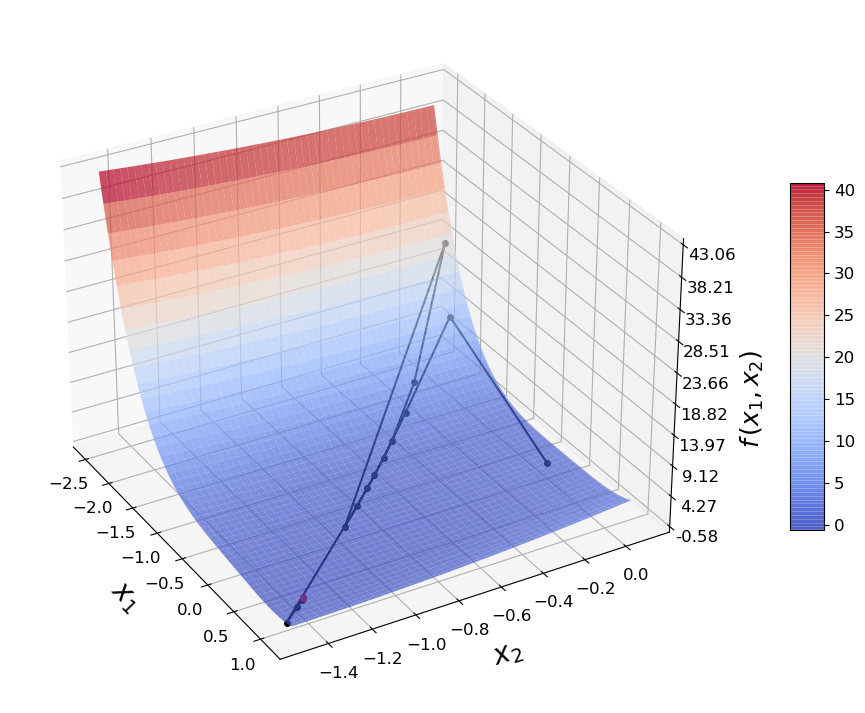
\includegraphics[scale=0.34]{Plot/func_d_standard_newton_x0_2_alpha=0.9_3d.png}}
		\caption{Contour plot and 3D plot for the function $f^{(d)}(x_{1},x_{2})$ where the intermediate points and the minimum point (in red) are obtained by using the standard Newton method with $\alpha=0.9$. The staring point considered in this case is $x_{0}=(0,0)^{T}$.}
		\label{Fig:func_d}
	\end{figure}
	
	
	\begin{table}[H]
		\centering
		\begin{tabular}{|c|c|c|c|}
			\hline
			k & $\| \textbf{x}_{k} - \textbf{x}^*\|_{2} $ & $f_{1}(\textbf{x}_{k}) - f_{1}(\textbf{x}^{*}) $ & $-\nabla f_{1}(\textbf{x}_{k})^{T}[\nabla^{2}f_{1}(\textbf{x}_{k})]^{-1} \nabla f_{1}(\textbf{x}_{k})$ \\
			\hline
			$0$ & $1.517$ & $1.582$ & $0.000$ \\
			$1$ & $8.014\times10^{-1}$ & $3.716$ & $-5.554$ \\
			$2$ & $3.959\times10^{-1}$ & $4.724\times10^{-1}$ & $-7.576\times10^{-1}$ \\
			$3$ & $1.232\times10^{-1}$ & $3.61\times10^{-2}$ & $-6.559\times10^{-2}$ \\
			$4$ & $1.717\times10^{-2}$ & $6.364\times10^{-4}$ & $-1.253\times10^{-3}$ \\
			$5$ & $4.011\times10^{-4}$ & $3.414\times10^{-7}$ & $-6.834\times10^{-7}$ \\
			$6$ & $2.275\times10^{-7}$ & $-4.435\times10^{-10}$ & $-2.171\times10^{-13}$ \\
			$7$ & $3.061\times10^{-9}$ & $-4.436\times10^{-10}$ & $-2.197\times10^{-26}$ \\
			\hline
		\end{tabular}
	\end{table}
	
		\begin{figure}[H]
		\centering
		\subfloat[][]{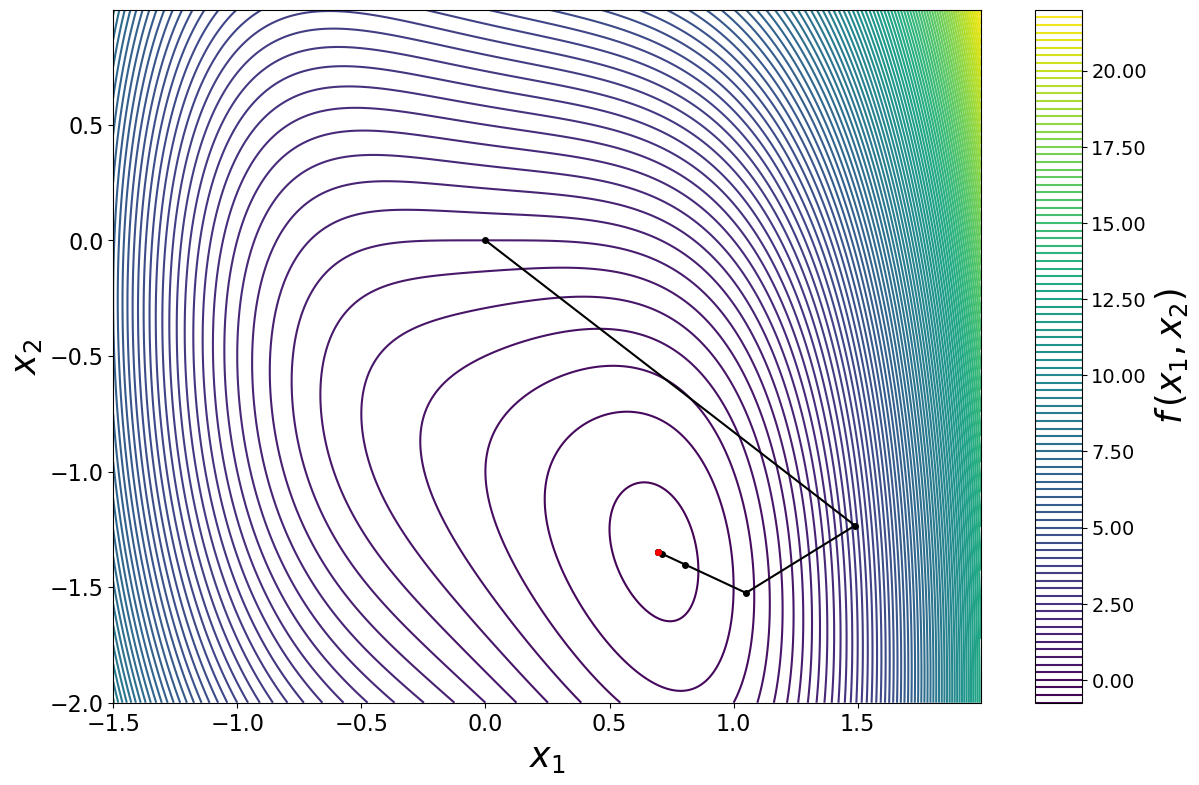
\includegraphics[scale=0.24]{Plot/func_d_newton_trustreg_contour.png}} \quad
		\subfloat[][]{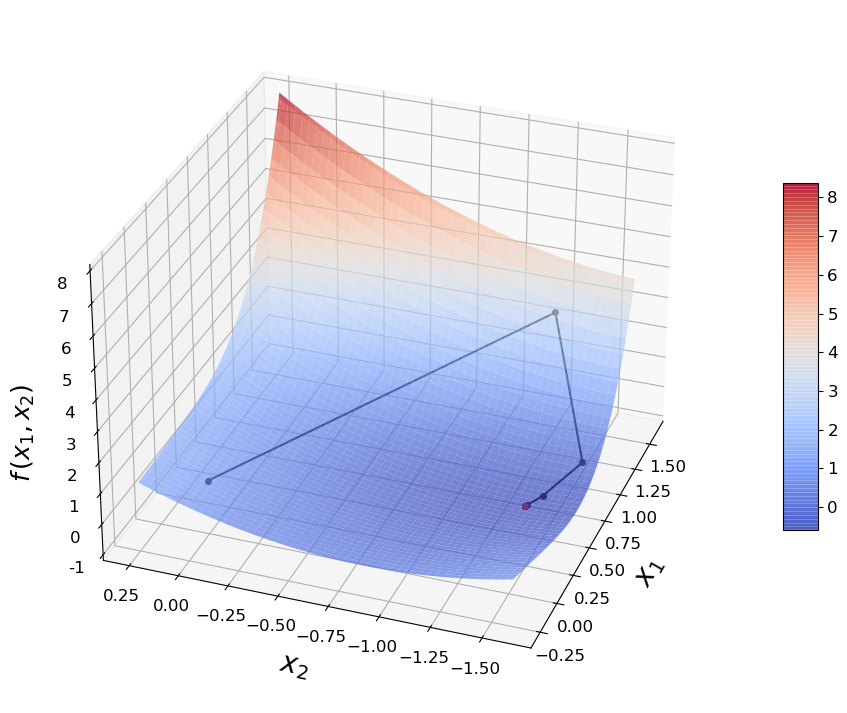
\includegraphics[scale=0.34]{Plot/func_d_newton_trustreg_3d.png}}
		\caption{Contour plot and 3D plot of the function $f^{(d)}(x_{1},x_{2})$ where the intermediate points and the minimum point (in red) are obtained by using the Newton method with the trust region approach. The starting point considered in this case is $x_{0}=(0,0)^{T}$.}
		\label{Fig:func_d}
	\end{figure}
	
\end{document}